% !TeX program = xelatex
\documentclass{tudelft-report} %[whitelogo]
\usepackage{algorithm}
\usepackage{algpseudocode}
\usepackage{amsmath}
\usepackage{amsthm}
\usepackage{blindtext}	% TODO Remove
\usepackage{changes}
\usepackage[nameinlink,capitalise]{cleveref}
\usepackage{enumitem}
\usepackage{amsbsy}
\usepackage{afterpage}
\usepackage{hyperref}
\usepackage[acronym]{glossaries} % toc does not work properly
\usepackage{siunitx}
\usepackage{subcaption} 
\usepackage{thmtools}
\usepackage{tikz}

\usetikzlibrary{automata,arrows,shapes}

\makeglossaries

\graphicspath{{./figures/}}

%% Glossary and Acronyms %%
%% List of acronyms %%
% Reference definition:
% - \newacronym[options]{label}{short}{long}
%	options: description, longplural, ...
%
% Reference usage:
% - \acrlong{label}  : displays the full text of the acronym
% - \acrshort{label} : displays the abbreviation
% - \acrfull{label}  : displays the full text followed by the abbreviation
% - \acrshortpl{label} : the plural of the abbreviation (similarly for acrlongpl and acrfullpl)

\newacronym{acr:dtp}{DTP}{Decision-Theoretic Planning}

\newacronym{acr:hmm}{HMM}{Hidden Markov Model}

\newacronym[longplural=Markov Decision Processes]{acr:mdp}{MDP}{Markov Decision Process}

\newacronym{acr:pomdp}{POMDP}{Partially Observable \acrshort{acr:mdp}}

\newacronym{acr:sdm}{SDM}{Sequential Decision Making}
%% Glossary Entries:
%
% Reference definition:
% \newglossaryentry{maths}
% {
% 	name=mathematics,
% 	description={Mathematics is what mathematicians do}
% }
%
% Reference usage:
% - \gls{ } Prints term lower case
% - \Gls{ } Prints term upper case
% - \glspl{ } Prints term plural lower case
% - \Glspl{ } Prints term plural upper case

\newglossaryentry{maths}{
	name={mathematics},
	description={Mathematics}
}

\newcommand\mat[1]{\pmb{#1}}
\newcommand\arr[1]{\pmb{#1}}
\DeclareMathOperator*{\argmax}{arg\,max}

%% Custom Definitions %%
\def\subsubsectionautorefname{Section}
\def\subsectionautorefname{Section}
\def\sectionautorefname{Section}
\def\chapterautorefname{Chapter}
\def\algorithmautorefname{Algorithm}

%\declaretheoremstyle[bodyfont=\normalfont]{normalbody}
%\declaretheorem[style=normalbody,name=Definition]{definition}
\theoremstyle{definition}
\newtheorem{definition}{Definition}
\newtheorem*{problem}{Problem Statement}

%% Pseudocode settings %%
\newcommand*\Let[2]{\State #1 $\gets$ #2}
\algrenewcommand{\algorithmiccomment}[1]{\hfill$\rhd$ #1} % Fix for comments in pseudocode

%% Title and Cover Pages %%

%% Use Roman numerals for the page numbers of the title pages and table of
%% contents.
\frontmatter

%% Uncomment following 16 lines for a cover with a picture on the lower half only
\title[tudelft-white]{Learning and Optimizing Probabilistic Models for Planning Under Uncertainty} %in Mobile Robot Navigation}
%\subtitle[tudelft-black]{Optional subtitle}
\author[tudelft-white]{R. van Bekkum}
\affiliation{Delft University of Technology}
\coverimage{figures/tank.jpg}
\covertext[tudelft-white]{
	\textbf{Cover Text} \\
	possibly \\
	spanning 
	multiple 
	lines
	\vfill
	ISBN 000-00-0000-000-0
}
\setpagecolor{tudelft-cyan}
%\makecover[split]

% TEMPORARY
\newcommand{\showoutline}[1]{
	\vspace{0.3cm}
	\hrule
	\vspace{0.3cm}
	{\large\textbf{PLANNED OUTLINE}:}
	\vspace{0.3cm}
	\hrule
	\vspace{0.3cm}
	{#1}
	\vspace{0.3cm}
	\hrule
	\vspace{0.3cm}	
}

\begin{document}

%% Include an optional title page.
\begin{titlepage}


\begin{center}

%% Insert the TU Delft logo at the bottom of the page.

% Print the title in cyan.
{\makeatletter
\largetitlestyle\fontsize{28}{94}\selectfont\@title										% TODO Change font size here
%\largetitlestyle\color{tudelft-cyan}\Huge\@title
\makeatother}

% Print the optional subtitle in black.
{\makeatletter
\ifx\@subtitle\undefined\else
    \bigskip
   {\tudsffamily\fontsize{22}{32}\selectfont\@subtitle}    
    %\titlefont\titleshape\LARGE\@subtitle
\fi
\makeatother}

%\rule{\textwidth}{.4pt}
%\medskip
%
%{
%\makeatletter
%\fontsize{23}{94}\selectfont\@title
%\makeatother
%}
%
%\medskip
%\rule{\textwidth}{.4pt}

%\bigskip
%\bigskip
%
%THESIS
%
%\bigskip
%\bigskip
%
%submitted in partial fulfillment of the\\requirements for the degree of
%
%\bigskip
%\bigskip
%
%MASTER OF SCIENCE
%
%\bigskip
%\bigskip
%
%in
%
%\bigskip
%\bigskip
%
%COMPUTER SCIENCE
%
%\bigskip
%\bigskip
%
%by
%
%\bigskip
%\bigskip
%
%Rob van Bekkum\\
%born in Hardinxveld-Giessendam, the Netherlands
%
%\bigskip
%\bigskip
%\bigskip
%\bigskip
%
%to be defended publicly on Tuesday July xx, 2017 at 10:00 AM.
%

%% OLD VERSION BEGIN %%

\bigskip
\bigskip

by
%door

\bigskip
\bigskip

%% Print the name of the author.
{\makeatletter
%\largetitlefont\Large\bfseries\@author
\largetitlestyle\fontsize{20}{26}\selectfont\@author
\makeatother}

\bigskip
\bigskip

to obtain the degree of Master of Science 

in Computer Science

at the Delft University of Technology,

to be defended publicly on Wednesday September 27, 2017 at 14:00.
% OLD VERSION END %%

\vfill

\begin{tabular}{lll}
    Student number: & 4210816 \\
    %Project duration: & \multicolumn{2}{l}{November 14, 2016 -- July xx, 2017} \\
    Thesis committee: & Dr.\ M.\ T.\ J.\ Spaan, & TU Delft, supervisor \\
        & Dr.\ Ing.\ J.\ Kober, & TU Delft \\												% TODO Update
        & Dr.\ M.\ Loog, & TU Delft 											% TODO Update
\end{tabular}
%% Only include the following lines if confidentiality is applicable.

%\bigskip
%\bigskip
%\emph{This thesis is confidential and cannot be made public until July xx, 2017.}
%\emph{Op dit verslag is geheimhouding van toepassing tot en met 31 december 2013.}

\bigskip
\bigskip
An electronic version of this thesis is available at \url{http://repository.tudelft.nl/}.

% ADDED
\bigskip
\bigskip

%\\[1cm]

%\centering{
\includegraphics{cover/logo_black}}

%\vfill
%
%\centering{
\includegraphics{cover/logo_black}}
%


\end{center}

\begin{tikzpicture}[remember picture, overlay]
    \node at (current page.south)[anchor=south,inner sep=48pt]{
        
\includegraphics{cover/logo_black}
%        Algorithmics Group\\
%        Department of Software Technology\\
%        Faculty EEMCS, Delft University of Technology\\
%        Delft, the Netherlands
    };
    \node[below right] at (current page.south)[anchor=south, inner sep=22pt] {\begin{minipage}{\textwidth}\centering\small
        Algorithmics Group\\
        Department of Software Technology\\
        Faculty EEMCS, Delft University of Technology\\
        Delft, the Netherlands
	 \end{minipage}};
    %\node[below right] at (current page.south)[anchor=south,inner sep=0pt] {Depart};
\end{tikzpicture}

\end{titlepage}



\chapter*{Preface}
\setheader{Preface}

% The thesis report contains a preface that explains the topic of the thesis, the context (institute or company), the main findings in a few lines and the names of the members of the thesis committee. The preface may end with a few acknowledgments, and completed with name and date.

In the last year of my master studies, I have had the opportunity to explore and gain insight into fields of research including planning, reinforcement learning and optimization that I was not familiar with at the start of this project.
This report documents the work on identifying the possibilities of automating the task of learning performance-maximizing Markov Decision Processes from data effectively, performed as a master thesis project in the Algorithmics Group of the Department of Software Technology of the EEMCS Faculty at the Delft University of Technology.

I would like to thank Bruno Lacerda, University of Birmingham, for the tips I got at the start of the project on the usage of the robot simulation software.
Especially, I would like to thank Matthijs Spaan for being my supervisor during this project in which the weekly meetings in which we could exchange ideas were very helpful.

\begin{flushright}
{\makeatletter\itshape
    \@author \\
    Delft, September 2017
\makeatother}
\end{flushright}

%
%\vspace{12pt}
%\noindent\fbox{\textbf{TODO:} Preface chapter needs to be updated: `Main findings in a few lines`}
%

\tableofcontents

%% Use Arabic numerals for the page numbers of the chapters.
\mainmatter

\chapter{Introduction}
\label{ch:introduction}

% 

\section{Motivation}
\label{sec:motivation}

There are several practical applications in which the (sequential) actions of systems are coordinated by decision makers or \textit{agents} to achieve long-term goals.
In particular these agents need to take into account the uncertainty in these systems that may be present in the form of action failures (e.g., a robot slipping), exogenous events (e.g., moving obstacles) and noisy observations.
To devise optimal plans for those systems whose dynamics are stochastic, \acrfull{acr:dtp} aims to account for uncertainty by exploiting the considerable structure these systems pose through the development of probabilistic models which reflect this uncertainty.
These probabilistic models serve as a system representation which describe a system's state and its evolution over time after a sequence of actions has been executed.
The advantage of having such (accurate) probabilistic models at one's disposal is that agents can act according to different policies derived from one and the same model to perform multiple tasks.

In recent years particularly \acrfullpl{acr:mdp} have become a significant popular formalism for modeling \acrshort{acr:dtp} problems. 
That is, first of all, due to their firm foundation in decision theory and successes of Markovian approaches in speech recognition and the closely-related field of \acrfull{acr:rl}.
Furthermore, over the years various computationally efficient solution techniques have been devised for obtaining optimal plans for \acrshort{acr:mdp} models which maximize expected value.
Considering the expediency of \acrshortpl{acr:mdp} for automated control, it seems worthwhile to investigate methods of developing accurate probabilistic models for the purpose of planning under uncertainty.

% New paragraph here

% Mainly applied approach in automated control involves hand-crafting a mathematical model as a system representation that can be used to represent the system's state and its evolution over time after a sequence of actions has been executed.
% Setting up such models is an important, difficult and time-costly process for human designer that might not always have (enough) expertise to craft a suitable model that can be used to plan for the execution of tasks.

\section{Problem Description}
\label{sec:problem-description}

The problem this thesis is concerned with is the development of probabilistic models, which are used for obtaining plans for automated control of systems whose dynamics are stochastic.
Setting up such models is an important, though difficult and time-costly process for a human designer that might not always have (enough) expertise to craft a suitable, well-generalizing model that can be used to plan for the execution of different tasks.
In practice, this problem is tackled by domain experts by iteratively tweaking the model parameters until the desired performance is achieved.

An alternative that one ought to consider, is that of applying \acrshort{acr:rl} techniques rather than planning algorithms.
However, although ideas from planning and \acrshort{acr:rl} are interchangeable, these techniques typically demand direct interaction with the environment which is something that cannot always be readily offered.
That is, \acrshort{acr:rl} techniques turn out as time-consuming and sometimes even riskful or dangerous when applied in real-world environments.
Those domains for which plans need to be formulated offline, demand the acquisition of probabilistic models which accurately define what constitutes the state of the system, reflect uncertainty through transition probabilities and some manner of specifying goals.%TODO Rewrite 'some manner of specifying goals'?

An attractive approach of bypassing the daunting and error-prone task of handcrafting probabilistic models, is that of automatizing the model development process by applying learning algorithms on data that describes the dynamics of the system.
For this approach the data is typically presented in the form of execution traces of the system operating in a real-world environment, which is collected in an exploration phase prior to the actual planning.
However, although one could obtain a model of the system by applying learning algorithms, the corresponding plans that are inferred from this model might not be effective when applied in a real-world environment.
First of all, this might be due to the parameters of the learning algorithm not being set properly, signifying the need for proper adjustment of these parameters.
Another possibility is that the gathered data is incomplete and so does not accurately describe the dynamics of the system.
In this case, one could choose to augment the data for those areas for which the training data is inadequate, although one should be aware that this is accompanied by a more cost-expensive model-learning process.
Therefore, in order to learn accurate probabilistic models, we are in need of a way of assessing the performance of a model accompanied by a method for identifying inadequacies due to incomplete data, while taking into account the corresponding cost of learning and evaluating these system models.

\section{Research Questions}
\label{sec:research-questions}
The problem statement as presented in the previous section yields the following main research question for this thesis:

\vspace{12pt}
\noindent\textbf{Main Research Question.} How can the task of obtaining a \acrfull{acr:mdp} that maximizes the yielded performance of executing plans that are derived from it, given a dataset about the system under consideration, be automated?
\vspace{12pt}

To answer this main research question, four research questions have been identified which are presented below.
The relevance of each of these research questions is discussed accordingly in the next paragraphs.

\vspace{12pt}
\noindent\textbf{Research Question 1.} Which learning algorithms exist that can be employed for learning \acrshortpl{acr:mdp} from data for systems involving uncertainty that require plans for automated control?
\vspace{0pt}

First off, to facilitate the formulation of plans for a system involving uncertainty, we need to obtain an \acrshort{acr:mdp} from the provided dataset.
Therefore, we should know what learning algorithms exist that can be employed to learn the parameters of an \acrshort{acr:mdp}.
Accordingly, we should identify the applications for which each of these algorithms are suited, but also what the shortcomings or vulnerabilities of each of these algorithms are.

\vspace{12pt}
\noindent\textbf{Research Question 2.} How should a performance measure be defined which can be used to fairly compare the value of different \acrshortpl{acr:mdp}?
\vspace{12pt}

As various \acrshortpl{acr:mdp} can be obtained for different parameter settings of the model learning algorithms, the need for a measure of performance for different \acrshortpl{acr:mdp} emerges.
That is, to establish which parameter settings yield an \acrshort{acr:mdp} that best reflects the underlying system for the tasks to be executed, we require a way to express and fairly compare the value of the learned \acrshortpl{acr:mdp}.

\vspace{12pt}
\noindent\textbf{Research Question 3.} How can the parameter space of model learning algorithms cost-effectively be explored towards a global maximizer with only limited knowledge about the system under consideration?
\vspace{12pt}

A model learning algorithm may yield different \acrshortpl{acr:mdp} depending on the selected parameter settings.
To establish the most appropriate \acrshort{acr:mdp} for the system under consideration, the performance yielded by multiple \acrshortpl{acr:mdp} should be compared.
As evaluating all possible parameter-settings would be cost-expensive, we need to investigate other ways of exploring the parameter space more cost-effectively.
This is under the assumption that we only have limited to no belief over which parameter-settings might work well for the system under consideration.

\vspace{12pt}
\noindent\textbf{Research Question 4.} How can the hierarchy of different abstraction levels be exploited to find a performance-maximizing \acrshort{acr:mdp} in a more cost-effective way?
\vspace{12pt}

Assessments of performance can be made at different levels of abstraction of the underlying system.
That is, we could examine how well an agent would perform a task only from the perspective of the \acrshort{acr:mdp} model, but also
from simulations or even the real world.
At the one hand abstracting from the real world typically yields a less accurate representation of the reality, although on the other hand assessing the performance from a more abstract level is accompanied by smaller computational costs.
Therefore it might be valuable to investigate how this could be exploited to achieve a more cost-effective optimization of the performance.

%\vspace{12pt}
%\noindent\textbf{Research Questions:}
%\begin{enumerate}[label=\textbf{\arabic*})]
%	\item Which methods exist for learning (probabilistic) models from data for a system involving uncertainty that requires plans for automated control?
%	\item How should a performance measure be defined that can be used to fairly compare the value of different \acrshortpl{acr:mdp}?
%	\item How can the hierarchy of different abstraction levels be exploited to find a performance-maximizing \acrshort{acr:mdp} in a more cost-effective way?
%\end{enumerate}

\section{Contribution}
\label{sec:contribution}

We propose a framework for automating the development of probabilistic models in the form of \acrshortpl{acr:mdp} by applying learning algorithms on data describing the dynamics of the system under consideration.
The data about the environment that is used by these learning algorithms is gathered prior to the model learning process in an exploration phase.
In order to obtain accurate probabilistic models for the system under consideration, the parameters of the used learning algorithm should be tweaked in such way to optimize the performance in the execution of its tasks.
%In order to obtain accurate probabilistic models for the system under consideration, the parameter-settings of the used model learning algorithm are iteratively tweaked towards a setting that maximizes the performance in the execution of the tasks expected to be performed.
To achieve this we pose the adjustment of the learning algorithm parameters as an optimization task to maximize the performance that follows from executing plans derived from learned \acrshortpl{acr:mdp}.
The optimization is performed by applying a technique known as Bayesian Optimization, so that we define a probability distribution over functions to model the performance measure and iteratively sample parameter-settings towards a global maximizer of the performance.

%To address model inadequacies that are due to incomplete data, we propose to incorporate the identification of insufficient exploration for the transitions from those states that are visited in the execution of obtained plans.
%That is, for those learned models for which the data was observed to be incomplete, the observations of the performance for the corresponding parameter-settings are modeled as noisy or uncertain.
%This serves the purpose of more cautious exploitation of those areas of the parameter space which mostly produce noisy observations of the performance measure.

To achieve a more cost-effective optimization, the parameter search space is first narrowed down by a pre-processing step.
In this step assessments of the model value are made on a more abstract level (i.e., based on the computed value function for an \acrshort{acr:mdp}).
The posterior that follows from this step is then used to define a prior over the true model value used for the following step.

In attempt to further improve the learned models, a post-processing step is performed that aims to identify and fix discrepancies between the model and the real-world.
This post-processing step increases the resolution for those areas of the state-space when it identifies the outcomes of actions in simulations do not match the learned transition probabilities.

The framework is applied, tested and evaluated for the domain of mobile robot navigation, as the robots in this domain oft to operate under significant uncertainty in their actions.
A solution in this context is a policy which maps discretized robot poses into fine-grained navigation actions so to move a mobile robot to a certain goal location.
Probabilistic models are acquired by applying unsupervised machine learning algorithms on execution traces (consisting of odometry data describing robot poses) obtained in an exploration phase.
The optimization of the model is based on the performance of acquired models in simulations, which is expressed in terms of the time that has passed to reach multiple goal locations.
Incomplete exploration data is here identified by inspecting the trajectories that are obtained from the execution of an optimal plan for an \acrshort{acr:mdp}.

% labeled as noisy uncertain observation of the performance of the model

% Discuss the learning and optimization routine: Automized method for learning probabilistic models in the form of MDPs by applying (machine) learning algorithms on exploration data. Optimization of the model by Bayesian Optimization based on performance in simulations.
% Identify incomplete exploration data about the environment by inspecting the observed trajectories and provide feedback on this from the optimization loop.
% Application to mobile robot navigation; A solution in this context is a policy that maps discretized robot poses into fine-grained navigation actions.

\section{Scope and Limitations}
\label{sec:scope-limitations}

First of all, we restrict ourselves to learning fully observable \acrshortpl{acr:mdp} from data.
However, this framework could possibly be extended to deal with applications where the states cannot be directly observed and should be inferred from observations.

Secondly, we note that all experiments and corresponding results are based on data that is solely obtained from simulations of a mobile robot.
Reasons for this are that we make the assumption that the environment is fully observable, which is typically not the case for real-world applications.
However, we should also note that the framework is not solely intended for the domain of mobile robot navigation.% and not having a real robot at hand, which would be too expensive and comes with its own technical challenges that are outside of our scope.

Finally, we focus on the domain of mobile robot navigation to evaluate and test our approach.
One of the important aspects to consider, is which data should be collected to describe the dynamics of the system to learn models from this data.
For our implementation we choose to collect data about the robot's poses from internal odometry, but for other applications we might not be able to describe the states and transitions of the system through a geometric model and may need other learning algorithms than the clustering algorithms we use for our application.
An example of such applications might be that of learning \acrshortpl{acr:mdp} for traffic light control \cite{wiering2004intelligent, delgado2011efficient}, in which, for instance, lane-turn probabilities could be learned from a data-set.
As a side note, this application seems particularly appropriate to be approached in combination with \acrshort{acr:rl} techniques, as it could adapt to the changes that occur over time.

% POMDPs: Restricted to MDPs, but could possible be extended to deal where the states are cannot be directly observed and should be inferred from observations.
% Field of application: We will discuss how the proposed method could be applied to other domains, although we will focus on the domain of mobile robot navigation to evaluate and test our method.

\section{Overview}
\label{sec:introduction-overview}

The framework that we propose is aimed at automating the development of probabilistic models for the purpose of automated control by agents through planning under uncertainty.
In the learning routine the plans are obtained through techniques founded in \acrlong{acr:dtp} in which probabilistic models are employed to achieve this.
In \autoref{ch:background} we make the type of problems that are faced in \acrshort{acr:dtp} concrete and review how specialized probabilistic models can be used by existing algorithms to acquire plans.
For the optimization of the parameters of learning algorithms we use a method known as Bayesian Optimization. In \autoref{ch:bayesian-optimization} we formally describe how this method works and how it is relevant to sequential decision making, supported by a number of successful applications for learning and planning.
In \autoref{ch:problem-related-work} we explore other existing techniques for the development of \acrshort{acr:mdp} models for systems involving uncertainty.
A solution to the problem we described, is proposed in \autoref{ch:methodology}, in which we put the theory and algorithms discussed in the earlier chapters together into an optimization routine.
To test and evaluate our solution we choose to make an implementation for the optimization of probabilistic models for the path planning of a mobile robot.
In \autoref{ch:experimental-results} we discuss the results obtained from testing the proposed solution with our implementation for mobile robot navigation.
Finally, in \autoref{ch:conclusions} we summarize and evaluate the proposed solution.

%
%\vspace{12pt}
%\noindent\fbox{\textbf{TODO:} Needs small updates, in Contributions and the chapter overview}
%%
\chapter{Decision-Theoretic Planning}
\label{ch:background}
% Introduction on what is Decision-Theoretic Planning
Automated \acrfull{acr:sdm} comprises the central problem of planning under uncertainty. 
\acrfull{acr:dtp} is concerned with the design of plans or \textit{policies} for settings in which uncertainty exists about the effects of actions, where the decision maker or \textit{agent} has incomplete information about the environment and its initial conditions, and where trade-offs need to be made between potentially conflicting objectives to determine an optimal course of action.
This chapter gives an introduction to the type of problems faced in \acrshort{acr:dtp} and explains how specialized probabilistic models can be used to solve these problems efficiently.
First of all, in \autoref{sec:problem-formulation} the goal of \acrshort{acr:dtp} and how the problems that are considered are generally approached is discussed.
Subsequently, \autoref{sec:system-representation} gives an overview of the probabilistic models that are used to make the structure of problems in \acrshort{acr:dtp} explicit.
Finally, in \autoref{sec:planning} some of the most common algorithmic planning techniques are discussed, which either learn a plan directly or through learning and solving a model.

\section{General Problem Formulation}
\label{sec:problem-formulation}
% Formulation of what kind of planning problems are considered in Decision-Theoretic Planning

The class of problems that are considered in \acrlong{acr:dtp} are those that require optimal stochastic control through the actions of decision maker(s), referred to as \textit{agent(s)}, in systems whose dynamics can be modeled as \textit{stochastic processes} \cite{Boutilier1999}.
The agent(s) in these systems sequentially need to choose from a set of actions that influence the system's behavior, consequently making the system switch from one state to another.
In these settings the system's current state and the agent's choice of action determines the probability distribution over the states the system might reach next.
In addition, the agent(s) might be uncertain about the system's current state, implying the need to infer from observations and making decisions based on probabilistic estimates of the system's state.

Typically the problems under consideration involve certain objectives to be achieved (e.g., tasks to be fulfilled) or properties to be satisfied (e.g., avoiding certain system states). 
Therefore the agent should decide on a optimal plan or \textit{policy} which makes it most likely for the system to reach its targets, while minimizing the risk of producing undesirable states and the accompanied costs of the policy.
To find such a policy for \acrlong{acr:sdm} problems, a typical approach is to first setup a probabilistic model of the system and then apply a \acrshort{acr:dtp} algorithm on this model.
This probabilistic model comprises a system representation which defines the state space in terms of a set of multi-valued features, the set of actions the agent may select together with the associated uncertainty defined by transition-probabilities, and a goal specification or performance metric typically expressed by means of a reward structure.

Overall \acrshort{acr:dtp} aims to devise planning algorithms for planning under uncertainty, a problem that is addressed in numerous different fields of research such as AI planning and control theory.
In particular difficulties arise when planning techniques are applied to determine courses of action for real-world settings, such as motion or path planning in robotics which both involve the possibility of action failures and disturbances caused by exogenous events.

\section{System Representations: Markov Models}
\label{sec:system-representation}
% Definitions of Markov Models relevant as probabilistic models for planning under uncertainty

As the class of problems considered in \acrshort{acr:dtp} oft to present considerable structure, there exist various proposed solutions for planning under uncertainty that apply model-based approaches.
This type of decision-theoretic planner uses a stochastic model of the environment in which the agent operates, which compasses the uncertainty that is associated with the agent's actions, observations and the exogenous events that might occur.
Typically the uncertainty is modeled by establishing a \textit{state space} for the system accompanied by a set of possible \textit{transitions} between the states that might be induced with a certain probability by an agent executing \textit{actions}.
The most common types of stochastic models that are used in \acrshort{acr:dtp} are called \textit{Markov Models} (sometimes also referred to as \textit{Markovian Models}), which has been motivated by their success in other fields such as speech recognition \cite{baker1992large, gales2008application, rabiner1989tutorial} and \acrfull{acr:rl} techniques \cite{Brafman2002}.
A Markov Model is a stochastic model in which the future states only depend on a limited number of prior observations. In fact, mostly processes or systems are modeled by Markov Models that satisfy the \textit{Markov Property}, which means that the state transitions are independent of any previous states or agent actions.

In the remainder of this section the most common types of discrete-state Markov Models are discussed one by one, starting from the fundamental models known as \textit{Markov Chains} in \autoref{subsec:markov-chains}, followed by their extension of \textit{\acrfullpl{acr:hmm}} in \autoref{subsec:hidden-markov-models}.
This again is followed by a discussion of the discrete-state Markov Models most relevant in \acrshort{acr:dtp}, being \textit{\acrfullpl{acr:mdp}} in \autoref{subsec:mdps} and their extension of \textit{\acrfullpl{acr:pomdp}} in \autoref{subsec:pomdps}.
Finally in \autoref{subsec:other-markov-models} other related state space models are briefly discussed.

\subsection{Markov Chains}
\label{subsec:markov-chains}
% Markov Chains: States and Transitions

The evolution of system or processes can be viewed as so-called \textit{time-series}, in which a set of data-points can be ordered using an underlying physical dimension, typically time \cite{barberBRML2012}.
Formally, time-series can be defined as a series $x_{a:b}$ of data-points, with $x_{a:b} \equiv x_a, x_{a+1}, \ldots, x_b$.
By means of these time-series, probabilistic models can be devised for real-world systems or processes, by introducing the notion of \textit{states} as a description of the system at a particular point in time or \textit{stage}.

On the basis of the class of Markov Models lies the simplifying assumption that each state is only dependent on a limited number of previous states.
Under this assumption a \textit{Markov Chain} (or \textit{Markov Process}) can be defined as a model of a series $q_{1:T}$ of transitions between states $q_i$ drawn from a state space $\mathcal{S} = \{s_1,\ldots,s_n\}$. The initial state $q_1$ of a Markov Chain typically is either fixed or drawn from $\mathcal{S}$ using a probability distribution over initial states.
For the states or variables of a Markov Chain, the earlier mentioned assumption implies the following conditional independence to hold:
\begin{equation}
	p(q_t \vert q_1,\ldots,q_{t-1}) = p(q_t \vert q_{t - L}, \ldots, q_{t-1})
\end{equation}
where $L$ is the so-called \textit{order} of the Markov Chain.
% See summary barberBRML2012

\begin{figure}[t!]
	\captionsetup[subfigure]{justification=centering}
	\centering
	\subcaptionbox{First-order Markov Chain.\label{fig:markov-chains-first-order}}{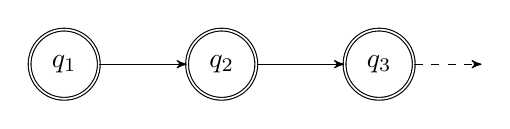
\begin{tikzpicture}[->,>=stealth',auto,node distance=2cm]
		\tikzstyle{every state}=[fill=white,draw=black,text=black,scale=1,double]	% thick
		\node[state] (s1) {$q_1$};
		\node[state] (s2) [right of=s1] {$q_2$};
		\node[state] (s3) [right of=s2] {$q_3$};
		\coordinate (con) at (0,2);
		\path
		(s1)
		edge node {} (s2)
		(s2)
		edge node {} (s3)
		(s3);
		\draw [->, dashed, shorten >=0pt] (s3) to[right] node[auto] {} ++(1.3,0)
		;
		\end{tikzpicture}} \quad
		\subcaptionbox{Second-order Markov Chain.\label{fig:markov-chains-second-order}}{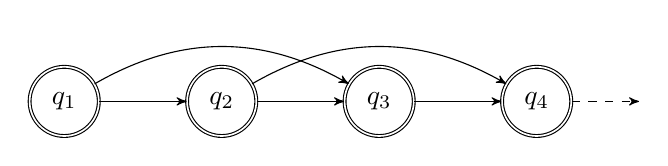
\begin{tikzpicture}[->,>=stealth',auto,node distance=2cm]
		\tikzstyle{every state}=[fill=white,draw=black,text=black,scale=1,double]	% thick
		\node[state] (s1) {$q_1$};
		\node[state] (s2) [right of=s1] {$q_2$};
		\node[state] (s3) [right of=s2] {$q_3$};
		\node[state] (s4) [right of=s3] {$q_4$};
		\path
		(s1)
		edge node {} (s2)
		(s2)
		edge node {} (s3)
		(s1)
		edge [bend left] node {} (s3)
		(s3)
		edge node {} (s4)
		(s2)
		edge [bend left] node {} (s4)
		;
		\draw [->, dashed, shorten >=0pt] (s4) to[right] node[auto] {} ++(1.3,0)
		;
		\end{tikzpicture}}
	\caption{Graphical representation of different types of Markov Chains.}
	\label{fig:markov-chains}
\end{figure}

As depicted in \autoref{fig:markov-chains}, Markov Chains of different order can be defined. \autoref{fig:markov-chains-first-order} exemplifying a first-order Markov Chain in which each state only depends on the previous state, and \autoref{fig:markov-chains-second-order} showing a second-order Markov Chain in which each state depends on the two prior states of the Markov Chain.
In the special case where the transition distribution is independent of the stage of the system, but solely on the prior state(s), one speaks of a \textit{stationary} or \textit{homogeneous} Markov Chain.

Though, mostly first-order Markov Chains as depicted in \autoref{fig:markov-chains-first-order}, which are said to satisfy the \textit{Markov Property}, are applied widely for modeling stochastic processes, such as physical phenomena and economic time-series \cite{bacciu2015probabilistic}.
In addition, mostly compact, stationary, discrete-time, finite-space Markov Chains are used, bearing in mind the computational adequacy of the model (i.e., the larger the state space and order, the more computational cost might be incurred).
Some concrete examples of practical applications include assessing the reliability and/or safety of appliances in engineering \cite{cochran2001generic, cronvall2009combining,el2008optimal}, modeling water flows \cite{parent1991stochastic}, or modeling loan defaults \cite{grimshaw2011markov} in the financial world (for an overview see \cite{pasanisi2012estimating}).

In these chains the state transition probabilities can be stored in an $n \times n$ transition matrix $\mat{A} = [a_{ij}]$ with each entry
\begin{equation}
	a_{ij} = p(q_{t+1} = s_i\vert q_t = s_j)
\end{equation}
denoting the probability of state $s_i$ following state $s_j$.
Similarly, the initial state probabilities can be recorded in an $n \times 1$ initial state vector $\arr{\pi} = [\pi_i]$ with each entry
\begin{equation}
	\pi_i = p(q_1 = s_i)
\end{equation} 
denoting the probability of state $s_i$ being the initial state of the model.
Putting these components all together, a discrete stationary first-order Markov Chain can be defined as a 3-tuple $\mathcal{M} = (\mathcal{S}, \mat{A}, \arr{\pi})$ with $\mathcal{S}$ as state space, $\mat{A}$ as transition matrix and $\arr{\pi}$ as initial state vector.

\subsubsection*{Fitting Markov Chains}
There exist efficient methods for fitting a discrete stationary first-order Markov Chain provided a collected dataset describing the evolution of a stochastic process either by applying likelihood maximization (e.g., see \cite{bacciu2015probabilistic, barberBRML2012, lee1968maximum, teodorescu2009maximum}) or Bayesian inference (e.g., see \cite{barberBRML2012, lee1968maximum, minka2003bayesian}).
These methods estimate the transition distribution to fit a Markov Chain on a collected sequence of time-ordered states. 

The first-mentioned approach of likelihood maximization, works by estimating the transition probabilities by counting the observed transitions in the state sequence.
That is, if we let $n_{ij}$ denote the number of observed transitions from state $s_j$ to state $s_i$, then the maximum-likelihood estimation of the corresponding transition probability is
\begin{equation}
	p(q_{t+1} = s_i\vert q_t = s_j) = \frac{n_{ij}}{\sum_j n_{ij}}
\end{equation}

The second-mentioned approach of Bayesian inference is more suitable for many real-life problems, for which state sequences are incomplete, i.e. states are recorded only for certain stages, meaning there might be gaps in-between.
This type of approach aims to make an estimation of the transition probabilities by adopting a prior for the transition matrix $\mat{A}$, a convenient choice being a factorized prior from the product of $n$ independent \textit{Dirichlet} distributions, one for each row $\mat{A}_j$ such that:
\begin{equation}
	p(\mat{A}) = \prod_{j} \text{Dir}(\mat{A}_j \vert \alpha_j)
\end{equation}
parametrized by a vector $\arr{\alpha}$ with $\alpha_j > 0$ \cite{pasanisi2012estimating,barberBRML2012}.

\subsection{Hidden Markov Models}
\label{subsec:hidden-markov-models}
% Hidden Markov Models: Observations (partially observable) 
% also called latent
% inference problems
% shortly discuss the succesful applications see \cite{barberBRML2012} speech recognition, object tracking, genetic sequence analysis and add citations to the corresponding works

The Markov Chain model discussed in \autoref{subsec:markov-chains} requires the modeled system or stochastic process to be fully observable, meaning that each of its states correspond directly to an observation.
However, it is not unusual to encounter real-world systems in which the states are assumed to be unobservable, though are correlated with observable events produced by the system.
These systems can be modeled by a \acrfull{acr:hmm} in which the states, typically referred to as \textit{hidden} or \textit{latent} variables $h_{1:T}$, are unknown.
Additionally this model consists of observations, typically referred to as \textit{observed} or \textit{visible} variables $v_{1:T}$, which are dependent on the hidden variables through an emission $p(o_t\vert h_t)$ graphically depicted in \autoref{fig:hmm}. All by all a stationary \acrshort{acr:hmm}
consists of the following parts:

\begin{itemize}
	\item a discrete set of $n$ attainable states $\mathcal{S} = \{s_1, \ldots, s_n\}$, i.e. the underlying \textit{state space}
	\item a set of $m$ possible observations, $\mathcal{V} = \{v_1, \ldots, v_m\}$, i.e. the \textit{observation space}
	\item an $n \times n$ transition matrix $\mat{A} = [a_{ij}]$ defining the models' \textit{transition distribution} in which $a_{ij} = p(h_{t+1} = s_i \vert h_t = s_j)$ is the probability of state $s_i$ following state $s_j$ ($s_i, s_j \in \mathcal{S}$)
	\item an $m \times n$ emission matrix $\mat{B} = [b_{ij}]$ defining the models' \textit{emission distribution} in which $b_{ij} = p(o_t = v_i \vert h_t = s_j)$ the probability of observing $v_i$ from state $s_j$ ($v_i \in \mathcal{V}$, $s_j \in \mathcal{S}$)
	\item an $n \times 1$ initial state array $\arr{\pi} = [\pi_i]$ in which $\pi_i = p(h_1 = s_i)$ is the probability of having $s_i$ as the initial state ($s_i \in \mathcal{S}$)
\end{itemize}
Putting all of these components together, a stationary \acrshort{acr:hmm} can be defined as a 5-tuple $\mathcal{M} = (\mathcal{S}, \mathcal{V}, \arr{\pi}, \mat{A}, \mat{B})$ with $\mathcal{S}$ as state space, $\mathcal{V}$ as observation space, $\arr{\pi}$ as initial state vector, $\mat{A}$ as transition matrix and $\mat{B}$ as emission matrix.

\begin{figure}[t!]
	\centering
	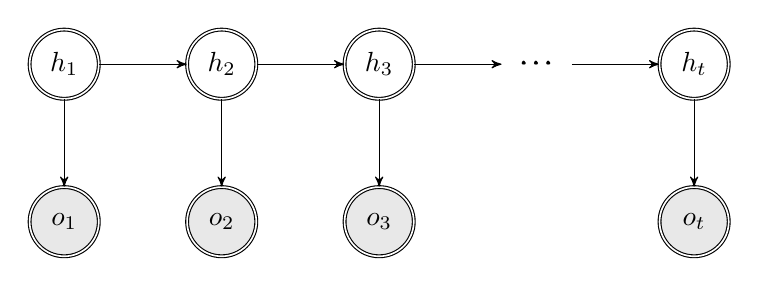
\begin{tikzpicture}[->,>=stealth',auto,node distance=2cm]
	\tikzstyle{every state}=[fill=white,draw=black,text=black,scale=1,double]	% thick
	\node[state] (h1) {$h_1$};
	\node[state] (h2) [right of=h1] {$h_2$};
	\node[state] (h3) [right of=h2] {$h_3$};
	\node[state, draw=none] (dots) [right of=h3] {$\pmb{\cdots}$};
	\node[state] (ht) [right of=dots] {$h_t$};
	\node[state,fill={rgb:black,1;white,10}] (o1) [below of=h1] {$o_1$};
	\node[state,fill={rgb:black,1;white,10}] (o2) [below of=h2] {$o_2$};
	\node[state,fill={rgb:black,1;white,10}] (o3) [below of=h3] {$o_3$};
	\node[state,fill={rgb:black,1;white,10}] (ot) [below of=ht] {$o_t$};
	\path
	(h1)
	edge node {} (h2)
	(h2)
	edge node {} (h3)
	(h3)
	edge node {} (dots)
	(dots)
	edge node {} (ht)
	(h1)
	edge node {} (o1)
	(h2)
	edge node {} (o2)
	(h3)
	edge node {} (o3)
	(ht)
	edge node {} (ot)
	;
	\end{tikzpicture}
	\caption{Graphical representation of an \acrshort{acr:hmm} with hidden states $h_t \in \mathcal{S}$ and observations $o_t \in \mathcal{V}$ for $t = 1:T$}
	\label{fig:hmm}
\end{figure}

In practice \acrshortpl{acr:hmm} have a wide range of applications. One example is that of object tracking in which inference algorithms for \acrshortpl{acr:hmm} are used to estimate the (unknown) position of objects by a sequence of observations \cite{caelli2001shape}. Another well-known application example of \acrshortpl{acr:hmm} is that in automatic speech recognition \cite{}. % TODO Elaborate (_little_ bit) and add citations

% Input figure showing graphical representation of an HMM
% Input subsubsection* about inference problems (see the three in thesis-plan, but also mention the other two)

\subsubsection*{Inference Problems}
The most notable inference problems for \acrshortpl{acr:hmm} are the following: %TODO Little introduction to this section?

\begin{description}
	\item[Evaluation] The \textit{Evaluation} or \textit{Likelihood Problem} is, given an \acrshort{acr:hmm} model $\mathcal{M}$ and an observation sequence $O = (o_1,\ldots,o_T)$ of length $T$, to determine $p(O\vert \mathcal{M})$, which is the likelihood of the observation sequence $O$ being produced by $\mathcal{M}$.
	\item[Optimal States] The \textit{Optimal State Sequence Problem} or \textit{Most Likely Hidden Path Problem} is, given an \acrshort{acr:hmm} model $\mathcal{M}$ and an observation sequence $O = (o_1,\ldots,o_T)$ of length $T$, to determine $H^\ast = \argmax_H p(H \vert O)$, i.e., finding the best state sequence $H^\ast = (h_1^\ast, \ldots, h_T^\ast)$ of length $T$ for the underlying Markov Chain.
	\item[Learning] The \textit{Learning Problem} is, given a set $\mathcal{O} = \{O_1, \ldots, O_k\}$ of independently and identically distributed observation sequences each of length $T$, to find an \acrshort{acr:hmm} $\mathcal{M}^\ast = \argmax_\mathcal{M} p(\mathcal{O}\vert \mathcal{M})$, i.e., maximizing the probability of the model having produced the observation sequences.
\end{description}
Other closely related inference problems are that of \textit{filtering} (inferring the present: $p(h_t\vert o_{1:t})$), \textit{prediction} (inferring the future: $p(h_t \vert o_{1:s})$ with $t > s$) and \textit{smoothing} (inferring the past: $p(h_t \vert o_{1:u})$ with $t < u$).

\subsection{Markov Decision Processes}
\label{subsec:mdps}

% MDPs: Actions --> Is a probabilistic model			% Driven by the actions of an agent
% 	(Exogeneous) events
% Policies

Although Markov Chains and \acrshortpl{acr:hmm} can be used to model the evolution of stochastic processes or systems, they do not allow for stochastic control through the actions of a decision maker or \textit{agent} which alter the state of the system.
The systems of interest in \acrshort{acr:dtp} however, involve agents that are assigned the task of influencing the behavior of the stochastic system by making sequential decisions to achieve certain goals.

% Actions
\acrfullpl{acr:mdp} extend on (stationary) Markov Chains by adding a finite set of actions $A$ available to the agent at each stage or \textit{decision epoch}.
Upon the agent choosing to perform an action $a \in A$, a state transition occurs in response to the action.
However, due to the uncertainty in the system, the actual transition that occurs might differ from the transition intended by the chosen action.
This uncertainty is captured by defining a probabilistic transition function $\delta: \mathcal{S} \times A \times \mathcal{S} \mapsto [0,1]$ which maps the combination of a current state and action to a probability of ending up in a certain next state.

% Reward structure
As the agent of an \acrshort{acr:mdp} aims to fulfill certain goals through the selection of actions, it requires some means of assessing which action is the best to pick.
The value measure used in \acrshortpl{acr:mdp} is defined by a mapping $R: \mathcal{S} \times A \times \mathcal{S} \mapsto \mathbb{R}$ from states and actions to real-valued \textit{rewards} (in case of added value) and/or \textit{costs} (in case of lost value).
Due to the uncertainty in the modeled system, typically the agent uses the \acrshort{acr:mdp}'s transition distribution (defined by transition function $\delta$) to compute expected values, and accordingly selects actions that maximize this quantity.

% Formal definition
Putting all of these components together, an \acrshort{acr:mdp} can be defined as a 5-tuple, $\mathcal{M} = (\mathcal{S}, s_0, A, \delta, R)$ with $\mathcal{S}$ as state space, $s_0 \in \mathcal{S}$ as the initial state, $A$ as finite set of possible actions, $\delta$ as probabilistic transition function and $R$ as reward function.

% Policies
In the context of \acrshort{acr:dtp}, \acrshortpl{acr:mdp} are used to find an optimal course of action, often referred to as a plan or \textit{policy}.
For an \acrshort{acr:mdp} the optimal policy typically means the policy that when applied by an agent, maximizes the expected value.
Although, one can also choose to express goals in alternative ways that does not require the specification of a reward function.
An example of this can be seen in \cite{bhatia2010sampling, lacerda2015optimal}, which replaces the reward function of the classic MDP-framework by a (co-safe) Linear Temporal Logic (LTL) formula to be satisfied.

\subsection{Partially Observable MDPs}
\label{subsec:pomdps}

% Observations: .. POMDP
% Reward Models and Value Functions

An extension of the traditional \acrshort{acr:mdp} models, are the \acrfull{acr:pomdp} models which account for uncertainty in the observations that are made by agents.
That is, while an \acrshort{acr:mdp} is used to model systems that are fully observable, in a \acrshort{acr:pomdp} the states are not observable and can only be inferred from the observations that are perceived.
In other words, we can intuitively view a \acrshort{acr:pomdp} as the combination of a \acrshort{acr:hmm} and an \acrshort{acr:mdp}.

As such, a \acrshort{acr:pomdp} can be defined as a 7-tuple $\mathcal{M} = (\mathcal{S}, s_0, A, \delta, \mathcal{O}, \Omega, R)$ with $\mathcal{S}$ as state space, $s_0 \in \mathcal{S}$ as the initial state, $A$ as finite set of possible actions, $\delta$ the transition function, $\mathcal{O}$ the observation space, $\Omega$ an emission or observation probability function and $R$ as reward function.
As the true state of a \acrshort{acr:pomdp} is unknown, the transition function $\delta$ is defined over beliefs of states, and accordingly a policy $\pi$ maps beliefs to actions.
The observation function $\Omega: \mathcal{S}\times A \mapsto \mathcal{O}$ defines the probability of observations from state-action pairs in the \acrshort{acr:pomdp} and is used to iteratively update the belief-state of an agent.

\subsection{Other Markov Models and Related State-Space Models}
\label{subsec:other-markov-models}
Apart from the discrete-state Markov Models that were discussed in this section, there exist numerous other types of Markov Models and closely related State-Space Models (SMMs), including among others the following:%, including continuous-state Markov Models (e.g., Linear Dynamical Systems with a Gaussian state-space \cite{Minka1999,barberBRML2012}) and other specialized variations. 

\begin{description}
	\item[Factored Markov Decision Process (FMDP)] An extension of the MDP model that allows for compact representation of states, transitions and rewards \cite{Degris2010}. In many real-life domains especially the state-space grows exponentially with the number of variables. Therefore FMDPs can be used to exponentially reduce the representation by means of a dynamic Bayesian network. The main drawback, however, is that finding the best policy becomes an NP-hard problem.
	\item[Multi-Agent \acrshort{acr:mdp} (MMDP)] An \acrshort{acr:mdp} model for systems that involve multiple decision makers. In this model each agent chooses an individual action with the goal of optimizing a joint reward. Other variations involving multiple agents are Decentralized \acrshortpl{acr:mdp} (Dec-MDPs) and \acrshortpl{acr:pomdp} (Dec-POMDPs), which differ from MMDPs in that the agents can only approximate the global state of the process by their own (local) observations \cite{Melo20111757}.
	%\item[Variable-order Markov Model (VOM)] To be determined 
	\item[Linear Dynamical System (LDS)] A continuous-state State-Space Model with linear dynamics, Gaussian state space and the assumption of hidden variables as in \acrshortpl{acr:hmm} \cite{Minka1999, barberBRML2012, Ghahramani2000}.
\end{description}
% TODO Extend each with sentence to explain the need for these models

As the remaining chapters only consider systems and processes that are modeled using discrete-state Markov Models, these variations will not be further discussed in more detail.

\section{Learning Optimal Policies}
\label{sec:planning}

In \acrshort{acr:sdm} problems typically the aim is to determine a policy that maximizes the total expected value obtained.
In algorithmic planning techniques a probabilistic model of the environment, which includes estimates of the transition probabilities and rewards, is used to obtain an optimal policy by exploring its state-space towards a goal.
On the other hand, in \acrfull{acr:rl} the optimal policy is learned while interacting with the environment and it is applied when one does not know the transition probabilities and rewards for its states upfront.
Both techniques have in common that they iteratively update estimations of a value function to derive a policy.
The main difference though is that in planning this progress is carried out based on simulated experience from a model, while in learning techniques this is based on real experience from executing agents in an environment \cite{sutton1998reinforcement}.
So, even when considering the differences, various solutions can be exchanged between planning and \acrshort{acr:rl} techniques.

In this section the various approaches for finding optimal policies are discussed, where the planning techniques are discussed in \autoref{subsec:model-based-planning}, and \acrshort{acr:rl} techniques are discussed in \autoref{subsec:reinforcement-learning}.

% Sutton and Barto (1998/2012) describe two approaches for rl solutions when the transition and reward functions are not known	(Learning the Structure of Factored Markov Decision Processes inReinforcement Learning Problems)
% See chapter 8.2, show an adapted version of the figure and explain advantages and disadvantages
% Explain the difference between planning and learning

\begin{figure}[t!]
	\centering
	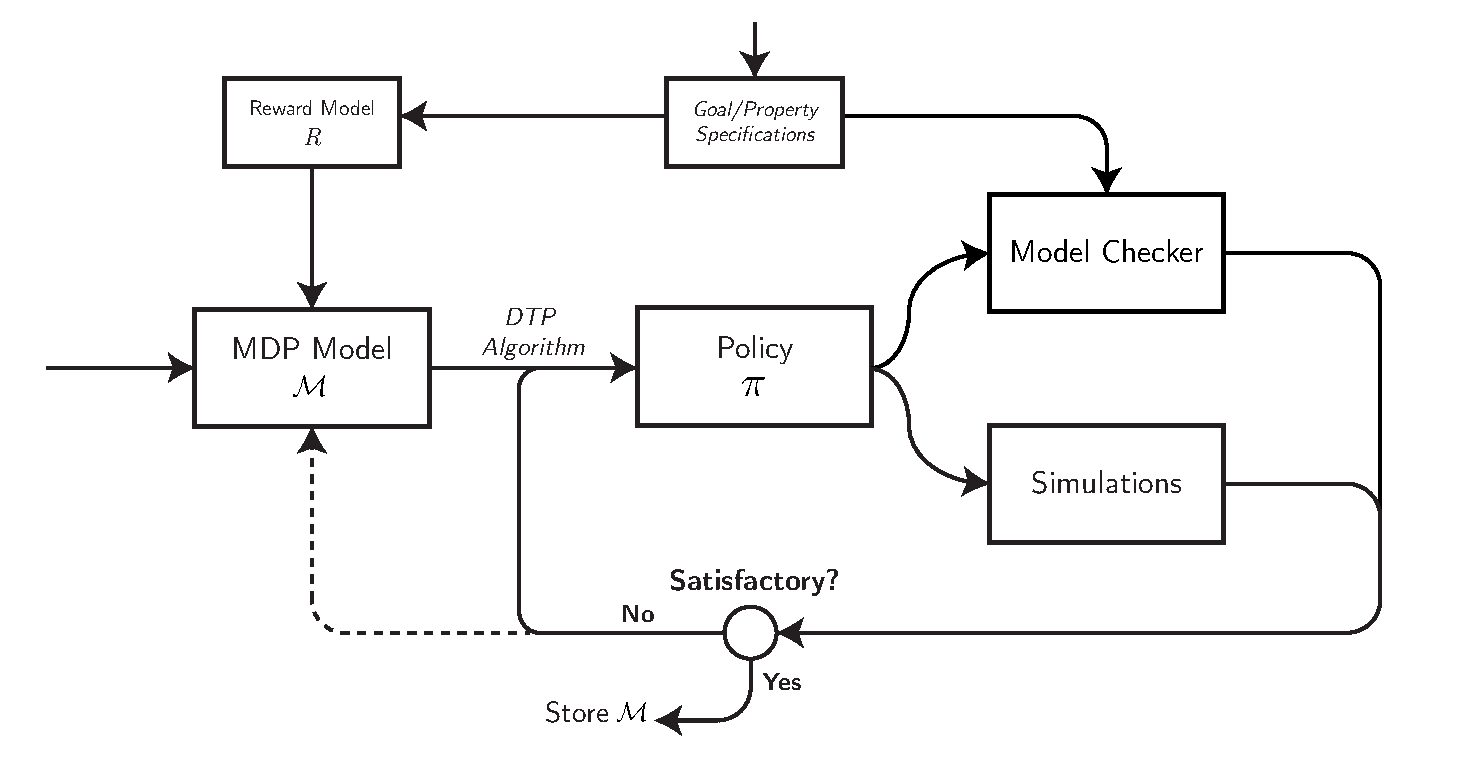
\includegraphics[width=\textwidth]{mdp-planning-diagram-v2}
	\caption{Block diagram of the generic routine employed in model-based MDP planning techniques.}
	\label{fig:model-based-routine}
\end{figure}

\subsection{Model-Based Planning Techniques}	% Also referred to as Indirect approaches
\label{subsec:model-based-planning}

In \acrshort{acr:dtp} the algorithms compute their plans or policies based on a probabilistic model of the environment.
Most common is to prepare an \acrshort{acr:mdp} and apply exact dynamic programming solutions to compute an optimal policy for that model.
The routine that is typically followed in MDP planning is depicted in \autoref{fig:model-based-routine}.
The state space, transition function and action space are usually handcrafted, based on expertise or trial and error.
The goal that should be fulfilled is translated into a reward model, mapping positive highly-valued rewards to desirable states and low rewards or costs to states that are not desirable or should even be avoided.
These parts together form the \acrshort{acr:mdp} which is fed to a planning algorithm which in this case is referred to as \textit{\acrshort{acr:mdp} solver}.
From this solver, a policy $\pi$ is obtained, which is usually evaluated by applying it in one or more simulations, rather than using it in a real-world environment.
Another option is to make use of automated model checking tools which can verify whether the policy will satisfy the set goals. % TODO Add citation to book about model checking from APS and Bruno
After evaluating the current policy, one may choose to stick with the current policy or adjust the settings of the solver or \acrshort{acr:mdp} model and obtain a new policy.

There are several options for the \acrshort{acr:mdp} solver, which compute an optimal policy by maximization of the expected value to be obtained.
In the remainder of this section various of these planning algorithms for \acrshortpl{acr:mdp} are discussed and evaluated.

\begin{algorithm}[]
	\caption{Value iteration}
	\label{alg:vi}
	\begin{algorithmic}[1]
		\Require{MDP $\mathcal{M} = (\mathcal{S}, s_0, A, \delta, R)$, discount factor $\gamma \in (0, 1)$, threshold $\xi > 0$}
		\Ensure{Optimal policy $\arr{\pi}^*: \mathcal{S} \mapsto A$}
		\State{Initialize $V_t: \mathcal{S} \mapsto \mathbb{R}$ arbitrarily for $t = 0$}
		\State $t \gets 0$
		\Repeat
		\State $t \gets t + 1$
		\ForAll{$s \in \mathcal{S}$}
		\State{$V_t(s) \gets \max_{a \in A} \left[\sum_{s' \in \mathcal{S}} \delta(s, a, s') \cdot \left[R(s, a, s') + \gamma \cdot V_{t-1}(s')\right]\right]$}
		\EndFor
		\Until{$\forall s \in \mathcal{S}: \lvert V_t(s) - V_{t-1}(s) \rvert \leq \xi$}
		\ForAll{$s \in \mathcal{S}$}
		\State $\arr{\pi}^*(s) \gets \text{arg max}_{a \in A} \left[\sum_{s' \in \mathcal{S}} \delta(s, a, s') \cdot \left[R(s, a, s') + \gamma \cdot V_{t}(s')\right]\right]$
		\EndFor
		\State\Return $\arr{\pi}^*$
	\end{algorithmic}
\end{algorithm}

\subsubsection*{Value Iteration}
\label{sec:value-iteration}

The most well-known algorithm for obtaining optimal policies from \acrshortpl{acr:mdp} is \textit{\acrfull{acr:vi}}, which is a synchronous dynamic programming solution which iteratively updates a value function $V: \mathcal{S} \mapsto \mathbb{R}$ until convergence given an MDP model $\mathcal{M} = (\mathcal{S}, s_0, A, \delta, R)$.
The updates are performed through so-called \textit{Bellman backups} based on the following Bellman equation:
\begin{align}
	V^*(s) &= max_{a \in A} \left[\sum_{s' \in \mathcal{S}} P(s' \vert s, a) \cdot \left[R(s, a, s') + \gamma \cdot V^*_{t}(s')\right]\right]	&\forall s \in \mathcal{S}
\end{align}
where $\gamma \in (0,1)$ is a discount factor which expresses the magnitude of preference of short-term solutions over long-term solutions. That is, the smaller the factor $\gamma$, the more important it is that goals are reached in as few steps as possible.

In \autoref{alg:vi}, it is shown how the \acrshort{acr:vi} algorithm can be used to obtain optimal policies for an MDP (based on the formulation in \cite{poole2010artificial}).
Intuitively, \acrshort{acr:vi} can be viewed as estimating the values starting from the goal-rewards and working backwards.
The initial values of the value function, stored in $V_0$, can be arbitrarily initialized, but to achieve faster convergence it is customary to do the initialization based on a rough estimation of $V^*$.
In every iteration, the estimates of the value function are updated by the backup operations based on the value in previous operations.
After a finite number of iterations the algorithm will converge (as is shown in \cite{puterman2014markov}) and after that point $V(s)$ gives us the maximum to be expected sum of rewards starting from a state $s \in \mathcal{S}$.
As can be seen in \autoref{alg:vi}, convergence is reached as soon as the change in value gets below a given threshold $\xi > 0$.
After such convergence has been reached, the policy can be defined by selecting the action $a \in A$ for each state $s \in \mathcal{S}$ that is most likely to maximize the collected rewards based on the value of $V_t(s)$.
All by all, the algorithm works well when the state space is relatively small, but for large state spaces more storage is required and it may take longer to reach convergence.

Note that an alternative formulation of the \acrshort{acr:vi} algorithm can be given that makes use of a $Q$-table instead of a value-function $V$.
In this formulation the entries $Q(s, a)$ are updated in each iteration for each state-action pair.
The optimal policy can then be obtained directly by selecting the action with the maximum value in the $Q$-table for each action, though it requires more storage compared to a value function.\newpage

\subsubsection{Asynchronous Value Iteration}
\label{sec:gs-value-iteration}

An adaptation of the traditional \acrshort{acr:vi} algorithm is \textit{asynchronous \acrshort{acr:vi}}, which is an asynchronous dynamic programming solution.
Almost all of the steps in asynchronous \acrshort{acr:vi} are the same except that rather than updating the value function $V: \mathcal{S} \mapsto \mathbb{R}$ for each state in each iteration, the function is updated only for a single state in each iteration in no particular order (or even randomized).
In the case of a fixed ordering, this algorithm is usually referred to as \textit{Gauss-Seidel \acrshort{acr:vi}}.
Compared to the traditional \acrshort{acr:vi} algorithm, the asynchronous adaptation requires less space and converges faster, especially when updates occur more often for most relevant states and the update ordering is adjusted carefully.

\textit{\acrfull{acr:rtdp}} \cite{barto1995learning} is a family of asynchronous \acrshort{acr:vi} algorithms which aim to find policies by performing updates and concurrently controlling the \acrshort{acr:mdp} (based on the policy corresponding to the latest estimate of the value function).
Opposed to traditional \acrshort{acr:vi}, where solving \acrshortpl{acr:mdp} with large state spaces is infeasible, RTDP algorithms often converge without examining all states.

% TODO POMDP Adaptation of Value Iteration See AI: A Modern Approach + Probabilistic Robotics

\begin{algorithm}[]
	\caption{Policy iteration}
	\label{alg:pi}
	\begin{algorithmic}[1]
		\Require{MDP $\mathcal{M} = (\mathcal{S}, s_0, A, \delta, R)$, discount factor $\gamma \in (0, 1)$}
		\Ensure{Optimal policy $\arr{\pi}^*: \mathcal{S} \mapsto A$}
		\State{Initialize $\arr{\pi}_0$}
		\State $t \gets 0$
		\Repeat
		\State Solve $\forall s \in \mathcal{S}$: $V_{\arr{\pi}_{t}}(s) \gets \sum_{s' \in \mathcal{S}} \delta(s, \arr{\pi}_t(s), s') \cdot \left[R(s, \arr{\pi}_t(s), s') + \gamma \cdot V_{\arr{\pi}_{t}}(s')\right]$
		\State $t \gets t + 1$
		\ForAll{$s \in \mathcal{S}$}
		\State $\arr{\pi}_t(s) \gets \argmax_{a \in A} \left[\sum_{s' \in \mathcal{S}} \delta(s, a, s') \cdot \left[R(s, a, s') + \gamma \cdot V_{\arr{\pi}_{t - 1}}(s')\right]\right]$
		\EndFor
		\Until{$\arr{\pi}_{t} = \arr{\pi}_{t-1}$}
		\State\Return $\arr{\pi}_t$
	\end{algorithmic}
\end{algorithm}

\subsubsection{Policy Iteration}
\label{sec:policy-iteration}

Another algorithm that is widely applied for obtaining policies from \acrshortpl{acr:mdp} is known as \textit{\acrfull{acr:pi}}. As shown in \autoref{alg:pi} \acrshort{acr:pi} starts off with an initial policy vector $\arr{\pi}_0$ which may be arbitrarily initialized, but preferably by an approximation of an optimal policy for the input MDP $\mathcal{M} = (\mathcal{S}, s_0, A, \delta, R)$ to achieve faster convergence.
Then in each iteration, first the value for each state is computed based on the latest policy $\arr{\pi}_t$, which comes down to solving a set of linear equations.
Solving this set of linear equations can be done by linear programming in (at most) $O(\lvert\mathcal{S}\rvert^3)$ time \cite{littman1995complexity}. 
An alternative approach, known as \textit{modified policy iteration}, is to solve these by applying a simplified form of value iteration in which the actions to select are already known for each state from the policy (i.e., $\arr{\pi}_t(s)$ for each $s \in \mathcal{S}$).
This step which is known as \textit{policy evaluation} is followed by a \textit{policy improvement} step in which the policy is greedily updated based on the latest value function $V_{\arr{\pi}}$.
This process is repeated until no improvements are possible and the policy stops changing.

Compared to \acrshort{acr:vi} the algorithm always converges in a finite number of iterations. However, solving the set of linear equations in each iteration is a more time-costly operation, especially for large state spaces.
That is, in \acrshort{acr:vi} each iteration takes $O(\lvert\mathcal{S}\rvert^2\cdot\lvert A\rvert)$ time, although one must note that the number of iterations is not finite, while \acrshort{acr:pi} finds an optimum in a finite number.\newpage

\begin{algorithm}
	\caption{Backwards induction}
	\label{alg:backwards-induction}
	\begin{algorithmic}[1]
		\Require{MDP $\mathcal{M} = (\mathcal{S}, s_0, A, \delta, R)$, horizon $h \in \mathbb{N}$}
		\Ensure{Optimal policy $\arr{\pi}^*: \mathcal{S} \mapsto A$}
		\State $t \gets h$
		\State $\forall s \in \mathcal{S}: V_h(s) \gets 0$
		\Repeat
		\State $t \gets t - 1$
		\ForAll{$s \in \mathcal{S}$}
		\State $V_t(s) \gets \max_{a \in A} \left[\sum_{s' \in \mathcal{S}} \delta(s,a,s') \cdot \left[R(s,a,s') + V_{t+1}(s')\right]\right]$
		\EndFor
		\Until{$t = 1$}
		\ForAll{$s \in \mathcal{S}$}
		\State $\arr{\pi}^*(s) \gets \argmax_{a \in A} \left[\sum_{s' \in \mathcal{S}} \delta(s,a,s') \cdot \left[R(s,a,s') + V_{1}(s')\right]\right]$
		\EndFor
		\State\Return $\arr{\pi}^*$
	\end{algorithmic}
\end{algorithm}

\subsubsection{Backwards Induction}
\label{sec:backwards-induction}

In the special case of a finite horizon \acrshort{acr:mdp} it is possible to obtain an optimal policy by applying \textit{backwards induction} \cite{chamie2015finite} shown in \autoref{alg:backwards-induction}.
As the name suggests the algorithm works backwards, starting from the last step $h$ and recursively using the value function of step $t + 1$ to compute that of step $t$.
Even though the algorithm works well when dealing with finite horizons, typically real world scenarios more often deal with infinite horizons for planning under uncertainty.

\subsubsection{Linear Programming}
\label{sec:linear-programming}

A less frequently applied approach is that of formulating the \acrshort{acr:mdp} as a \acrfull{acr:lp} and solving it using so-called \textit{simplex} methods.
Following this approach, an \acrshort{acr:lp} formulation for an MDP $\mathcal{M} = (\mathcal{S}, s_0, A, \delta, R)$, as explained in \cite{pazis2012non}, is:

%\begin{align}
%\max_{\lambda} &\sum_{s \in \mathcal{S}}\sum_{a \in A}\sum_{s' \in \mathcal{S}} \lambda(s, a) \delta(s, a, s')R(s, a, s') &\nonumber\\
%\text{s.t.} &\sum_{a' \in A} \lambda(s', a') = \mu_0(s) + \gamma \sum_{s \in \mathcal{S}}\sum_{a \in A} \lambda(s,a)\delta(s,a,s')	&\forall s' \in \mathcal{S} \\
%&\lambda(s,a) \geq 0 &\forall s \in \mathcal{S}, \forall a \in A \nonumber
%\end{align}
\begin{align}
\min_{V} &\sum_{s' \in \mathcal{S}} \mu_0(s) \cdot V(s) &\nonumber\\
\text{s.t. } &V(s) \geq \sum_{s' \in \mathcal{S}} \delta(s, a, s') \left[R(s,a,s') + \gamma\cdot V(s')\right]	&\forall s \in \mathcal{S}, \forall a \in A
\end{align}
where $\mu_0: \mathcal{S} \mapsto [0,1]$ is a probability distribution over the states.

From the solution $V^*$ of this \acrshort{acr:lp} formulation, a policy $\arr{\pi}^*$ can be obtained by letting $\arr{\pi}^*(s) = \argmax_{a \in A} \sum_{s' \in \mathcal{S}} \delta(s, a, s') \left[R(s,a,s') + \gamma\cdot V(s')\right]$ for each state $s \in \mathcal{S}$. This primal formulation optimizes a value function $V$, but alternatively the policy can be optimized directly by considering the dual formulation (see \cite{littman1995complexity}).
Comparing \acrshort{acr:lp} solutions to the specialized \acrshort{acr:vi} and \acrshort{acr:pi} solutions, the latter typically hold more promise for efficient solutions than general-purpose \acrshort{acr:lp} algorithms, although the \acrshort{acr:lp} scale better to larger \acrshort{acr:mdp} planning problems.

\subsection{Reinforcement Learning Techniques}
\label{subsec:reinforcement-learning}

\acrfull{acr:rl} techniques work on real experience based on which they update the behavior of the agent that is defined by an action-selection policy. To do this they require direct interaction with the environment to obtain experience and update value function estimations accordingly during execution.
Although most planning algorithms cannot be used for learning problems, learning algorithms can be used for planning problems as they can make use of simulated experience.
There are several techniques that exist, of which the most common ones are discussed in the remainder of this section.

\newpage

\subsubsection{Q-Learning}
\label{sec:q-learning}

Q-Learning is a model-free reinforcement learning technique which discovers an action-selection policy by learning estimates of the optimal Q-values of an \acrshort{acr:mdp}.
The technique starts off with a Q-table $Q$, which is arbitrarily initialized, containing the Q-values $Q(s,a)$ for each state-action pair $(s,a)$.
In each point in time, the agent for which the Q-Learning technique is applied, is assumed to be in a certain state $s$, and chooses a next action $a$ to execute based on the current Q-value estimates.
After executing an action the agent ends up in a new state $s'$ and observes a certain reward $r$.
The Q-table is then updated accordingly based on the following update rule:
\[
Q(s, a) = Q(s, a) + \alpha \Big[r + \gamma \max_{a'} Q(s',a') - Q(s, a)\Big]
\]
where $\alpha \in (0,1)$ is the learning rate and $\gamma \in (0, 1)$ the discount factor.
The learning rate expresses the rate at which newly acquired information overrides the old information in the Q-table.
Over time the estimates in the Q-table will improve such that the revenue is maximized.
A near-optimal policy can then be constructed by selecting the action with the highest Q-value from the Q-table for each state.

% 
% Also note that it can be used for planning

\subsubsection{SARSA}
\label{sec:sarsa}

\begin{algorithm}
	\caption{SARSA}
	\label{alg:sarsa}
	\begin{algorithmic}[1]
		\Require{MDP $\mathcal{S}, A, \alpha, \gamma$}
		\Ensure{Optimal policy $\arr{\pi}^*: \mathcal{S} \mapsto A$}
		\State Initialize $Q: \mathcal{S} \times A \mapsto \mathbb{R}$ arbitrarily
		\Repeat
		\State Pick $s \in \mathcal{S}$ arbitrarily
		\State $a \gets \pi[s]$ %TODO
			\Repeat
			\State 
			\Until{$s$ is terminal}
		\Until{$Q$ converged}
		\State\Return $\arr{\pi}^*$
	\end{algorithmic}
\end{algorithm}

Another algorithm, similar to Q-Learning, is known as SARSA.
While Q-Learning is an off-policy method which learns the value of the optimal policy, SARSA is an on-policy method which learns the value of the policy it currently follows in order to iteratively improve this policy.
In each iteration, it takes the action yielded by its policy and observes
\chapter{Bayesian Optimization}
\label{ch:bayesian-optimization}
This chapter elaborates upon a method known as Bayesian optimization, which is used to automate the process of optimizing the parameters of an unknown objective.
First \autoref{sec:bayesian-optimization-problem} introduces the optimization tasks this method is aimed at and how these are relevant to \acrshort{acr:sdm} problems.
Subsequently, in \autoref{sec:bayesian-optimization-algorithm} the optimization method is formally described.
In \autoref{sec:bayesian-optimization-prior-acquisition} the configurable parts of the method are discussed, considering both advantages and disadvantages of available options.
Finally, in \autoref{sec:bayesian-optimization-applications} a number of applications of Bayesian optimization in the field of planning under uncertainty are discussed, serving as an overview of the method's successes in this field.

% More applications:
%https://www.cs.ox.ac.uk/people/nando.defreitas/publications/BayesOptLoop.pdf

\section{Problem Formulation}
\label{sec:bayesian-optimization-problem}

One of the problems that is faced in the field of optimization is that of maximizing a nonlinear, real valued \textit{objective function} $f: \mathcal{X} \mapsto \mathbb{R}$ on a domain $\mathcal{X} \subset \mathbb{R}^m$ ($m \geq 1$).
Formally, to find a global maximizer $x^\ast \in \mathcal{X}$ for which:
\begin{equation}
	x^\ast = \argmax_{x \in \mathcal{X}} f(x)
\end{equation}
In particular the problem turns out to be a common bottleneck when dealing with an objective function that is unknown and expensive to evaluate in terms of the required computational resources.
As an example, one could think of finding the hyper-parameters for a neural network which maximize the performance, where each single evaluation of a set of parameters requires one to train the neural network and assess the performance on a huge dataset.

Although this problem of optimizing expensive functions can be found in many different contexts, it is foremost a problem in sequential decision theory. 
That is, typically one can only hope to estimate objective functions of \acrshort{acr:sdm} problems in AI planning and reinforcement learning through expensive simulations \cite{Brochu2010, Ghahramani2015}.

A naive approach for optimizing the objective would be to evaluate a set of (random) combinations of parameters and see which parameter-settings seem to give the best results.
This approach however, usually requires expert knowledge and might demand a large number of function evaluations that do not necessarily provide new information about the parameter-space.
The method known as \textit{Bayesian optimization}, described in \autoref{sec:bayesian-optimization-algorithm}, improves on these naive approaches by making predictions about which regions of the parameter-space are expected to give the best results and hence limiting the number of function-evaluations.

\section{Algorithm Description}
\label{sec:bayesian-optimization-algorithm}

\textit{Bayesian optimization} is a powerful method for finding the maximum of a typically unknown, expensive, nonlinear objective function, while aiming to minimize the number of objective function evaluations and avoiding local maxima \cite{Brochu2010}.
This method first requires one to set a prior $p(f)$ over the objective function $f$, representing the belief about the space of plausible objective functions.
Then, the algorithm starts off by gathering a small set of initial sample-observation pairs of samples $x \in \mathcal{X}$ and corresponding objective values $y = f(x) + \varepsilon$.
These pairs are then stored in a set $\mathcal{D}_{1:t} = \{(x_i, y_i) \mid i = 1 \ldots t\}$ (i.e., the \textit{evidence set}) where we let $x_i$ denote the $i$th sample and $y_i = f(x_i) + \varepsilon_i$ the corresponding $i$th observation with noise $\varepsilon_i$.

% Posterior / Surrogate Function
The algorithm then derives a posterior distribution $p(f \vert \mathcal{D}_{1:t})$ which is, according to Bayes' Theorem, said to be proportional to the likelihood $p(\mathcal{D}_{1:t} \vert f)$ and the prior $p(f)$ for the first $t$ gathered observations, s.t.:
\begin{equation}
	p(f \vert \mathcal{D}_{1:t}) \propto p(\mathcal{D}_{1:t} \vert f) \cdot p(f)
\end{equation}
This posterior can be viewed as an estimation of the objective function $f$, referred to as a \textit{surrogate function}.
% It does so by applying Bayes' Theorem, which states that the posterior probability $P(M \vert E)$ of a model $M$ given evidence $E$ is proportional to the likelihood $P(E \vert M)$ of $E$ given $M$

% Acquisition function
To decide on which $x \in \mathcal{X}$ to sample and gather a new observation $f(x)$ from next, a so-called \textit{acquisition function} $u: \mathcal{X} \mapsto \mathbb{R}$ is used, which assigns a certain utility to evaluating $f$ at some particular $x \in \mathcal{X}$ given the evidence set $\mathcal{D}$ at that point.
This acquisition function should be defined such that it captures a correct balance between \textit{exploration} (to sample from areas with high uncertainty) and \textit{exploitation} (to sample from areas likely to improve on prior observations). For this reason many different classes of acquisition functions exist, which are discussed in little more detail in \autoref{sec:bayesian-optimization-prior-acquisition}.

% General Formulation Algorithm

\begin{algorithm}
	\caption{Bayesian Optimization (General Formulation) \label{alg:bayesian-optimization}}
	\begin{algorithmic}[1]
		\Require{Domain $\mathcal{X} \subset \mathbb{R}^m (m \geq 1)$, prior $p(f)$ and acquisition function $u: \mathcal{X} \mapsto \mathbb{R}$}
		\Let{$\mathcal{D}_0$}{$\emptyset$} \Comment{$\mathcal{D}$ is the evidence set}
		\For{$t \gets 1, 2, \ldots$}
			\Let{$x_t$}{$\argmax_{x \in \mathcal{X}} u(x \vert \mathcal{D}_{1:t-1})$} \Comment{Acquisition based on posterior $p(f \vert \mathcal{D}_{1:t})$}%\Comment{Retrieve the next sample}
			\Let{$y_t$}{$f(x_t) + \varepsilon_t$}  %\Comment{Record a new observation of $f$}
			\Let{$\mathcal{D}_{1:t}$}{$\mathcal{D}_{1:t-1} \cup \{(x_t, y_t)\}$} \Comment{Augment $\mathcal{D}$ with the new evidence}
			\State Update the prior $p(f)$ and posterior $p(f \vert \mathcal{D}_{1:t})$
			\State \textit{Break} when satisfactory \Comment{Stop condition defined by implementation}
		\EndFor
		\State \Return{$\argmax_{(x_i, y_i) \in \mathcal{D}} y_i$}
	\end{algorithmic}
\end{algorithm}

The general formulation of the Bayesian Optimization is presented in \autoref{alg:bayesian-optimization}.
For an implementation of the algorithm still three components need to be defined, which are the domain $\mathcal{X}$ of $f$, the prior over $f$, and last of all the acquisition function $u$.

\section{Choice of Prior and Acquisition Function}
\label{sec:bayesian-optimization-prior-acquisition}
In order to apply Bayesian optimization there are two major choices that need to be made, which are those of the prior distribution over the objective and the acquisition function. In this section the different options and corresponding considerations that need to be made for these two components are elaborated upon.

\subsection*{Prior Distributions}
\label{sec:bayesian-optimization-prior}
In Bayesian optimization the most common choice for the prior distribution is a \acrfull{acr:gp}, which is typically well-suited as it accounts for the uncertainty associated with each prediction.
Another important aspect that makes a \acrshort{acr:gp} a convenient choice for the prior distribution is that it induces a posterior distribution over the objective function that is analytically tractable.
Intuitively a \acrshort{acr:gp} can be viewed as a prior which assumes that similar inputs result in similar outputs.
For an objective function $f$, the \acrshort{acr:gp} defines a Gaussian probability distribution over $f(x)$ for each $x$, so that a \acrshort{acr:gp} can be expressed as a probability distribution over functions:
\begin{equation}
	P(f(x) \vert x) = \mathcal{N}(\mu(x), \sigma^2(x))
\end{equation}
where $\mathcal{N}$ denotes a normal distribution, while $\mu$ and $\sigma$ denote mean and standard deviation respectively.
By this definition, a \acrshort{acr:gp} can be viewed as a function that returns the mean and variance of a normal distribution over the possible values of $f$ at $x$. A \acrshort{acr:gp} as prior over an objective function $f$ is typically denoted as: 
\begin{equation}
\label{eq:gp}
f \sim GP(m(\cdot), K(\cdot, \cdot))
\end{equation}
so that the \acrshort{acr:gp} is completely specified by a mean function $m$ and a \textit{kernel} function $K$ defining the covariance.
The mean function $\mu$ is typically initialized by a constant mean, usually zero, due to the assumption that all points in the parameter space are equally likely and because the conditional mean can still be flexibly specified by the kernel function $K$ \cite{kawaguchi2015bayesian}.

The choice of the kernel or covariance function of the \acrshort{acr:gp} determines the smoothness of the estimations on the performance and confidence intervals of unexplored samples in the parameter space.
According to the various literature in the field of Bayesian Optimization the most common kernels are said to be the \textit{squared exponential} (also known as \textit{radial basis function (RBF)} or Gaussian) kernel and Mat\'ern kernel.
However, the squared exponential kernel turns out unrealistically smooth for practical applications \cite{snoek2012practical} and therefore would require properly selecting its hyper-parameters.
The Mat\'ern kernel serves as a more flexible class, where the hyper-parameters allow tweaking the distance at which there are almost no effects from previous samples and the rate at which these effects decrease, for which a reoccurring kernel appears to be an automatic relevance determination (ARD) Mat\'ern 5/2 kernel for machine learning applications \cite{snoek2012practical, kawaguchi2015bayesian}.


%\begin{itemize}
%	\item \acrfull{acr:gp}
%	\item Wiener Process
%\end{itemize}


\subsection*{Acquisition Functions}
\label{sec:bayesian-optimization-acquisition}
% Examples acquisition function: PMAX, IEMAX, MPI, MEI, (GP-)UCB, GP-Hedge
% TODO Introduction
Let us define $f(x^+)$ as the `best' observation, corresponding to the sample $x^+ = \argmax_{x_i \in x_{1:t}} y_i$ when considering the first $t$ samples.

% TODO "Best-known acquisition functions:"
\begin{description}
	\item[\acrfull{acr:mpi}] This acquisition function selects the next sample to maximize the probability of improvement, which is the sample $x \in \mathcal{X}$ so that:
	$$P(f(x) \geq f(x^+) + \xi)$$
	where $\xi \geq 0$ is a trade-off parameter.
	\begin{description}
		\item[Advantages] description
		\item[Disadvantages] description
	\end{description}
	\item[\acrfull{acr:mei}] description
	\begin{description}
		\item[Advantages] description
		\item[Disadvantages] description
	\end{description}
	\item[\acrfull{acr:gp-ucb}] description
	\begin{description}
		\item[Advantages] description
		\item[Disadvantages] description
	\end{description}
\end{description}

Others possible acquisition functions that are used in Bayesian optimization are PMAX, IEMAX and GP-HEDGE. % TODO

\section{Applications of Bayesian Optimization to Planning Problems}
\label{sec:bayesian-optimization-applications}

% TODO Write out completely, this is just a short overview
Most interesting applications that involve or are closely related to \acrshort{acr:dtp}:

In \cite{MartinezCantin2009}, Bayesian optimization is applied for a mobile robot that adaptively plans a path while maximizing the information it obtains from observations about its own location and the location of navigation landmarks in the environment.
The objective/cost function $C$ is parametrized by a policy-vector $\pi$ and approximations for selected samples are made by different functions over the belief-states of the \acrshort{acr:pomdp}.
Typically, estimating the belief-state is an expensive problem, typically carried out through SLAM algorithms in robotics.
Therefore, to minimize computational cost, a Bayesian optimization algorithm is applied with the choice of a \acrshort{acr:gp}-prior over $C$ and where new samples are acquired using an \acrshort{acr:mei} acquisition function.

In \cite{Moldovan2012}, ... (SAFE-MDP)

In \cite{martinez2007active}, ... (Robot Planning and Exploration under uncertainty)

%\subsection{Extensions on Bayesian Optimization}
%\label{sec:bayesian-optimization-extensions}
%\blindtext

\chapter{Problem Formulation and Related Work}
\label{ch:problem-related-work}

\section{Problem Formulation}
\label{sec:problem-formulation}

In \acrshort{acr:dtp} it is common to make use of a (compact) probabilistic model of the environment.
However, devising an optimal model for a specific system or process can be a daunting and error-prone task, when considering the wide range of possibilities while wanting a compact and computation-cost efficient model.

\section{Learning Probabilistic Models from Execution Traces}
\label{sec:learning-state-spaces}

\textbf{Iterative Adjustment of Probabilities}:
\begin{itemize}
	\item Likelihood maximization for Markov Chains/MDPs, which generalizes to Baum-Welch for HMMs/POMDPs
	\item Bayesian Inference (see section 2.2.1)
	\item Gradient-Ascent
\end{itemize}

\begin{figure}[]
	\centering
	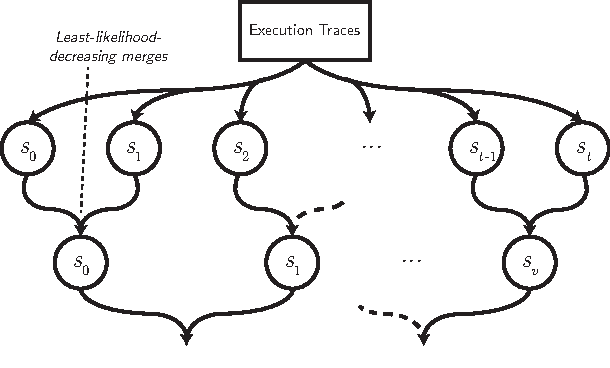
\includegraphics[width=0.8\textwidth]{model-merging-bfmm}
	\caption{State Merging}
	\label{fig:state-merging}
\end{figure}

\noindent \textbf{State Merging}:
\begin{itemize}
	\item Best-First Model Merging \cite{stolcke1994best}
	\item State Merging by Trajectory Clustering \cite{nikovski2000learning}
\end{itemize}

\noindent The other related work...

\section{Bayesian Reinforcement Learning}
\label{sec:bayesian-reinforcement-learning}

% https://people.eecs.berkeley.edu/~avivt/BRLS_journal.pdf
.....

% TODO;s
%% Fitting Markov Chains/MDPs:
	% Refer back to section 2.2.1:
	% - likelihood maximization
	% - Bayesian inference/optimization
%% Fitting HMMs/POMDPs:
	% ITERATIVE ADJUSTMENT OF PROBABILITIES:
	% - Baum-Welch Algorithm
	% - Gradient-Ascent in Likelihood
	% STATE MERGING
	% - Best-first
	% - Trajectory clustering
%% Reinforcement Learning: Online Model Learning

%% However, most of the previous works assume the state-space of the probabilistic model to be known.

%\section{Bayesian Reinforcement Learning}
%\label{sec:bayesian-reinforcement-learning}

% 

%
%\section{Overview}
%\label{sec:related-work-overview}
%
%% 
\chapter{Methodology and Setup}
\label{ch:setup}

% 

\begin{itemize}
	\item Introduction
	\item Explain full algorithm idea?
\end{itemize}

\section{Application}
\label{sec:application}

% 

\begin{itemize}
	\item Mobile robot navigation
	\item Why this application?
	\item Generalization possible to other applications?
\end{itemize}

\section{Exploration Phase}
\label{sec:exploration-phase}

% 

\begin{itemize}
	\item Obtain a dataset of observations, for our application this concerns data about attainable positions of the robot that will be controlled
	\item Under the assumption such a dataset is not yet available to us, this dataset is retrieved in an exploration phase
	\item In this exploration phase, the robot should explore the environment and periodically record information about its current position while aiming to visit all the locations of importance
	\item This exploration phase is (preferably) only carried out once
	\item To obtain a dataset for our tests the exploration phase is carried out in a robot simulator. Should also explain what data is obtained in this exploration.
	\item The overall algorithm is tested for multiple maps/(office-like) environments, which might differ in their dimensions, number of obstacles or `openness'.
	\item To take into account dynamically changing environments to some extent, there are also doors that will be open or closed as time passes.
	\item The simulations are carried out in the Morse simulator, in which the exploration is carried out by an agent that randomly navigates an environment.
\end{itemize}

\section{State Space Acquisition}
\label{sec:state-space-aggregation}

% 

\begin{itemize}
	\item Using exploration data
	\item Unsupervised machine learning to obtain states for an MDP model (various possible methods possible: e.g., kmeans, gmm)
	\item Unknown parameter $\delta$ of the unsupervised machine learning algorithm to be optimized
\end{itemize}

\section{Model and Policy Acquisition}
\label{sec:model-policy-acquisition}

% 

\begin{itemize}
	\item State space obtained as described in previous section
	\item Transition function obtained based on exploration data and state space through the likelihood maximization approach.
	\item For our application the actions are fixed and can either be \textsc{NORTH}, \textsc{EAST}, \textsc{SOUTH}, \textsc{WEST} which makes the robot navigate in the corresponding direction.
	\item Rewards
	\item Timesteps
	\item Policy (various possible `solvers': value iteration, policy iteration)
\end{itemize}

\section{Bayesian Model Optimization}
\label{sec:bayesian-model-optimization}

% 

\begin{itemize}
	\item Optimization of the unknown $\delta$ parameter of the machine learning algorithm for state space aggregation
	\item Evaluation by simulations of the found policy for the given $\delta$ parameter
	\item ...
\end{itemize}

\begin{figure}[t]
	\centering
	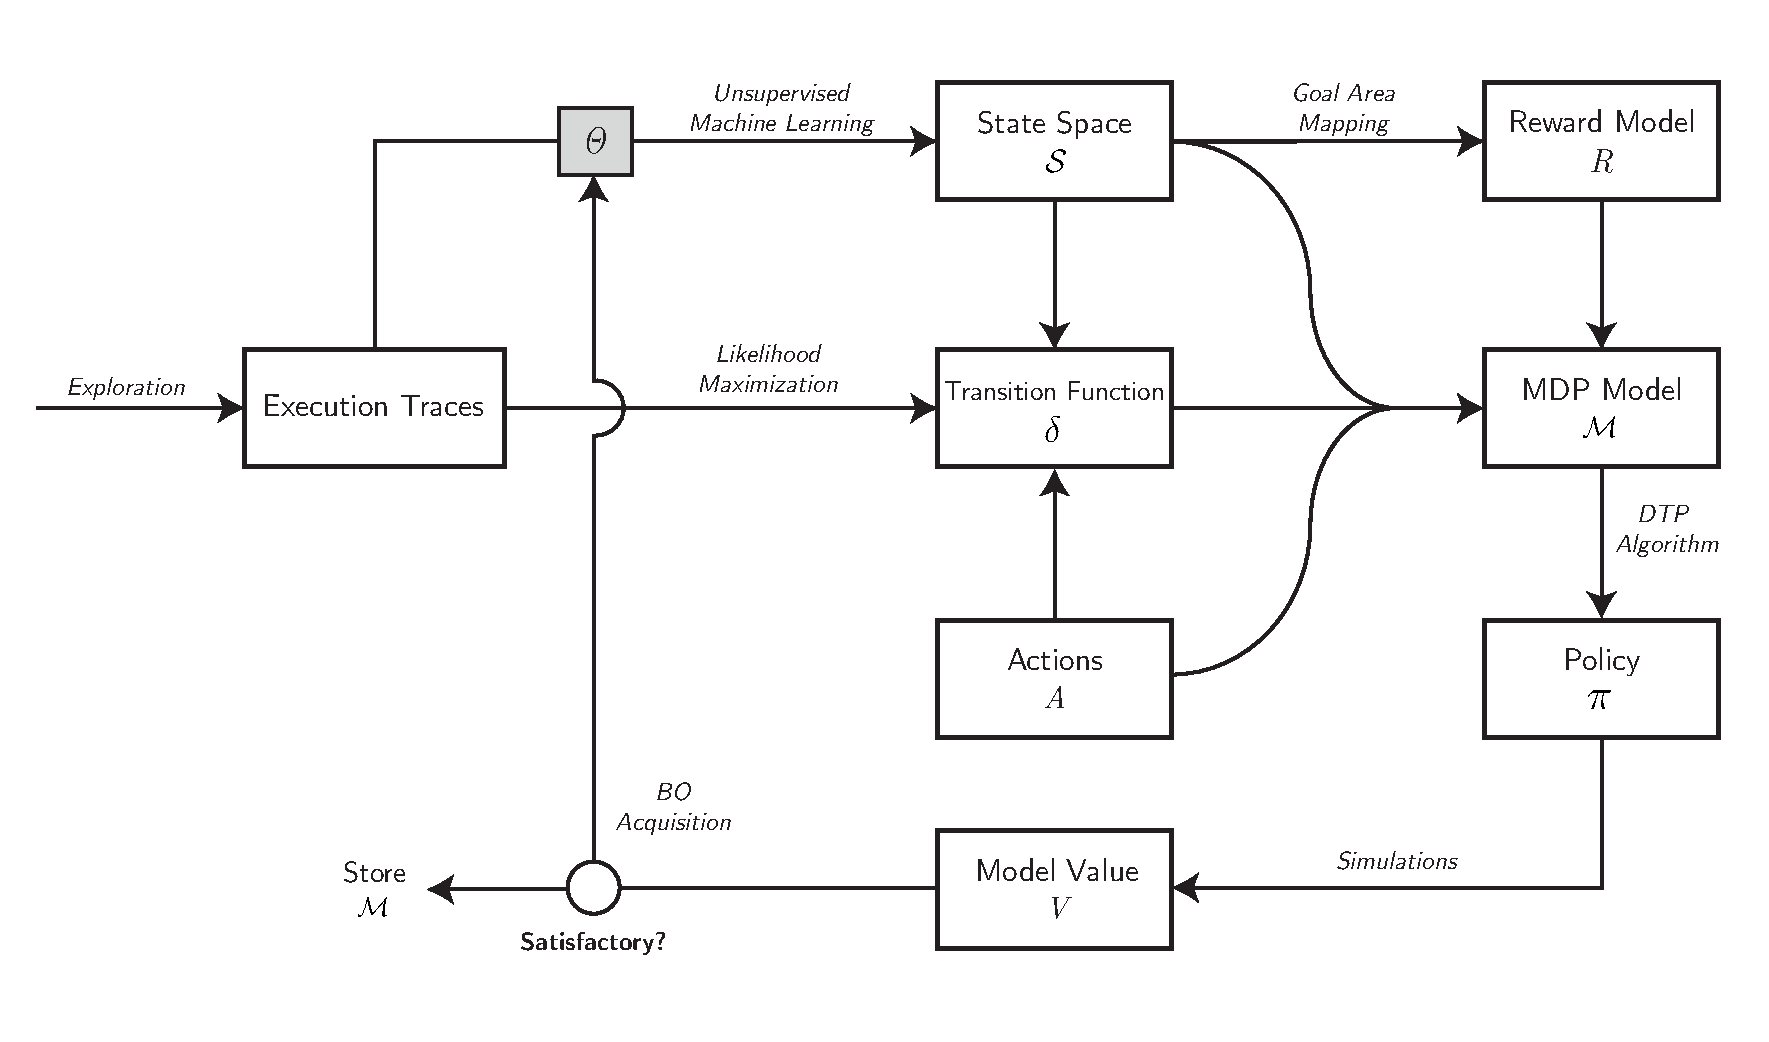
\includegraphics[width=\textwidth]{learning-cycle-complete-v2}
	\caption{Learning Cycle.}
	\label{fig:learning-cycle-complete}
\end{figure}


%% Use letters for the chapter numbers of the appendices.
\appendix

%\input{appendix-a}

% Acronyms and Glossary
\printglossary[type=\acronymtype]
%\printglossary

\bibliography{references}

\end{document}

% Using the order described here: http://academia.stackexchange.com/questions/5569/where-in-a-thesis-should-a-glossary-be-positioned

%TODO Check for consistent spelling, probably update glossary and check for use of dashes and change words to reach consistency
